\section[API-Usability-Verbesserungsvorschläge]{Vorschläge zur Verbesserung der API-Usability von SeqAn}
\label{sec:seqan-api-usability-vorschlaege}

In dem vorangegangenen Unterkapitel habe ich meine Theorie über die Entstehung und Auswirkungen von Entwurfsentscheidungen in SeqAn vorgestellt. Basierend auf den gefundenen Usability-Problemen und Strategien lassen sich Verbesserungsvorschläge erarbeiten, die ich in diesem Unterkapitel vorstelle. 

Dazu entwickle ich \textit{Maßnahmen}, die unterschiedliche Usability-Probleme teilweise oder praktisch vollständig lösen. Bei der Formulierung nehme ich keine Rücksicht auf die Abwärtskompatibilität der SeqAn-API. Dieses Vorgehen ist durch den VIP-Förderantrag (siehe \sref{sec:rahmenbedingungen}) abgedeckt und dank der eng angebundenen SeqAn-Anwender (siehe \sref{sec:seqan-kunden}) auch mit weniger Rücksichtnahme möglich.

%Die Abwärtskompatibilität etablierter APIs ist zwar ein wichtiges Qualitätsmerkmal \citep[vgl.][]{Fowler:2002ds,Bloch:2006jk}, jedoch angesichts der schlechten SeqAn-Usability kaum umsetzbar.

\subsection{Bewertung von Fatalität und Aufwand}

\begin{comment}
Einordnung nach den folgenden Eigenschaften des Usability-Problems:

\begin{itemize}
\item Die \emph{betroffene Partei} - also sind API-Entwickler oder API-Awender von der Designentscheidung betroffen.
\item Die \emph{Frequenz}, mit der man von einer Designentscheidung konfrontiert wird.
\item Die \emph{Schwierigkeit} des Umgangs mit einer Designentscheidung.
\end{itemize}

Zur Bewertung der \textit{Fatalität} \citep{Nielsen:1994tx} der gefundenen API-Usability-Probleme habe ich die Arbeit von \cite{Stylos:2006td} als Grundlage genommen und um zwei angepasste Faktoren aus der klassischen Usability-Forschung \citep{Nielsen:1994tx,Sarodnick:2006vc} erweitert.

\begin{description}
  \item[Betroffene Partei] \citep{Stylos:2006td} \\
  Sind API-Entwickler, API-(End-)Anwender oder Produktanwender betroffen?
  
  \item[Frequenz] \citep{Stylos:2006td,Nielsen:1994tx} \\
  Wie oft tritt dieses Problem auf?
  
  \item[Einfluss] (\cite{Nielsen:1994tx}; von \cite{Stylos:2006td} als \textit{Schwierigkeit} bezeichnet) \\
  Wir stark werden die betroffenen Parteien beeinflusst?
  
  \item[Persistenz] \citep{Nielsen:1994tx} \\
  Wird die betroffene Partei nur beim erstmaligen oder bei jedem Auftreten gestört?
  
  \item[Markteinfluss] \citep{Sarodnick:2006vc} \\
  Liegt ein Problem vor, das den kommerziellen Erfolg des Produkts grundsätzlich gefährdet?
\end{description}

%Aus dem besser erforschten Gebiet der (Nicht-API-)Usability kommt noch eine weitere Dimension dazu, die von \cite{Nielsen:1994tx} als \emph{Persistenz} bezeichnet wird. Persistenz beschreibt, ob ein Usability-Problem bei erneutem Auftreten auch immer wieder aufs neue als störend empfunden wird. Darüber hinaus schlagen \cite{Sarodnick:2006vc} \emph{Markteinfluss} als boolesche Eigenschaft vor. Diese Eigenschaft ist lediglich relevant, wenn die Nicht-Behebung eines Problems kommerzielle Folgen, z.B. durch Nicht-Verkauf des Produkts, wahrscheinlich macht.
\end{comment}

Für die Priorisierung einer Maßnahme sind die Schweregrade (\textit{Fatalitäten}) der adressierten Usability-Probleme und der Maßnahmendurchführungsaufwand zu ermitteln. Je höher die Gesamtfatalität und je geringer der Aufwand sind, desto höher ist die Priorität einer Maßnahme. Leider kann die Gesamtfatalität einer Reihe von Usability-Problemen nicht einfach durch Addition ermittelt werden \citep{Kahlert:2011wr}.

Bereits die valide Ermittlung der Fatalität eines jeden einzelnen Usability-Problems ist nicht einfach, denn dazu müssten praktisch alle Probleme in einer längeren Beobachtung überprüft worden sein. Schließlich definiert sich die Fatalität u.a. über die Eigenschaft \textit{Persistenz} \citep{Nielsen:1994tx}. Ob ein Usability-Problem dauerhaft, oder nur bei den ersten Erscheinungen Schaden anrichtet, kann aber nur so bestimmt werden.

Angesichts dieser Schwierigkeiten und meiner Beobachtung, dass sich praktisch alle Usability-Probleme auf \code{apiua://code/-9223372036854774824}, \code{apiua://code/-9223372036854775455} und \code{apiua://code/-9223372036854775441} auswirken, habe ich mich dazu entschlossen, die Gesamtfatalität und den Aufwand für jede Maßnahme nur grob zu schätzen.

Für die Schätzung der Gesamtfatalität habe ich mein, im Rahmen der wissenschaftlichen Literaturstudie erworbenes Wissen und die Phänomene meiner gefundenen Usability-Probleme genutzt. Ich verwende dabei die zur Gesamtfatalität inverse Metrik \textit{Kosten} mit der Ordinalskala: \textit{gering}, \textit{mittel} und \textit{hoch}.

Für die Schätzung der Kosten verwende ich dieselbe Ordinalskala wie folgt:
\begin{itemize}\itemsep1pt\parskip0pt\parsep0pt
  \item gering: < 1 Personenmonat
  \item mittel: >= 1 Personenmonat und < 4 Personenmonate
  \item hoch: >= 4 Personenmonate
\end{itemize}



\subsection{Maßnahmenkatalog}

Der im Folgenden dargestellte Maßnahmenkatalog listet alle gefundenen Usability-Probleme auf. Hinter jedem Usability-Problem sind die Maßnahmen genannt, welche die jeweiligen Usability-Probleme (teilweise) lösen sollen. Im Anschluss an diesen Katalog beschreibe ich die einzelnen Maßnahmen.

\begin{itemize}
  \item[\codebullet{apiua://code/-9223372036854774828}] \textbf{\codetext{apiua://code/-9223372036854774828}} 
  \begin{itemize}\itemsep1pt\parskip0pt\parsep0pt
    \item[\codebullet{apiua://code/-9223372036854774829}] \codetext{apiua://code/-9223372036854774829}: \textit{Frameworkumbau}
    \item[\codebullet{apiua://code/-9223372036854775633}] \codetext{apiua://code/-9223372036854775633}: \textit{STL-Angleichung, Dokumentation}
  \end{itemize}
   
  \item[\codebullet{apiua://code/-9223372036854774915}] \textbf{\codetext{apiua://code/-9223372036854774915}}  
  \begin{description}  
    \item[\codebullet{apiua://code/-9223372036854775117}] \textbf{\codetext{apiua://code/-9223372036854775117}}
    \begin{description}\itemsep1pt\parskip0pt\parsep0pt
      \item[\codebullet{apiua://code/-9223372036854775116}] \codetext{apiua://code/-9223372036854775116}: \textit{Inkonsistenzbeseitigung}
      \item[\codebullet{apiua://code/-9223372036854775057}] \codetext{apiua://code/-9223372036854775057}: \textit{Intransparenzbeseitigung}
      \item[\codebullet{apiua://code/-9223372036854774846}] \codetext{apiua://code/-9223372036854774846}: \textit{Inkonsistenzbeseitigung}
    \end{description}

    \item[\codebullet{apiua://code/-9223372036854775448}] \textbf{\codetext{apiua://code/-9223372036854775448}}
    \begin{description}\itemsep1pt\parskip0pt\parsep0pt
      \item[\codebullet{apiua://code/-9223372036854774860}] \codetext{apiua://code/-9223372036854774860}: \textit{Shortcuts}
      \item[\codebullet{apiua://code/-9223372036854774861}] \codetext{apiua://code/-9223372036854774861}: \textit{Shortcuts, Inkonsistenzbeseitigung}
      \item[\codebullet{apiua://code/-9223372036854775567}] \codetext{apiua://code/-9223372036854775567}: \textit{Dokumentation}
      \item[\codebullet{apiua://code/-9223372036854775623}] \codetext{apiua://code/-9223372036854775623}: \textit{Inkonsistenzbeseitigung}
      \item[\codebullet{apiua://code/-9223372036854775533}] \codetext{apiua://code/-9223372036854775533}: \textit{Shortcuts, Inkonsistenzbeseitigung}
    \end{description}
        
    \item[\codebullet{apiua://code/-9223372036854775237}] \textbf{\codetext{apiua://code/-9223372036854775237}}
    \begin{description}\itemsep1pt\parskip0pt\parsep0pt
      \item[\codebullet{apiua://code/-9223372036854775280}] \codetext{apiua://code/-9223372036854775280}: \textit{Dokumentation}      
      \item[\codebullet{apiua://code/-9223372036854775544}] \codetext{apiua://code/-9223372036854775544}: \textit{Dokumentation}

      \item[\codebullet{apiua://code/-9223372036854775279}] \codetext{apiua://code/-9223372036854775279}: \textit{keine Lösung}
      \item[\codebullet{apiua://code/-9223372036854775405}] \codetext{apiua://code/-9223372036854775405}: \textit{Dokumentation}
    \end{description}

    \item[\codebullet{apiua://code/-9223372036854775413}] \codetext{apiua://code/-9223372036854775413}: \textit{Dokumentation}
  \end{description}

  \item[\codebullet{apiua://code/-9223372036854775404}] \textbf{\codetext{apiua://code/-9223372036854775404}}
  \begin{description}\itemsep1pt\parskip0pt\parsep0pt
    \item[\codebullet{apiua://code/-9223372036854775572}] \codetext{apiua://code/-9223372036854775572}: \textit{Dokumentation}
    \item[\codebullet{apiua://code/-9223372036854775581}] \codetext{apiua://code/-9223372036854775581}: \textit{Dokumentation}
    \item[\codebullet{apiua://code/-9223372036854775577}] \codetext{apiua://code/-9223372036854775577}: \textit{Dokumentation}
    \item[\codebullet{apiua://code/-9223372036854775504}] \codetext{apiua://code/-9223372036854775504}: \textit{Dokumentation}
    \item[\codebullet{apiua://code/-9223372036854775271}] \codetext{apiua://code/-9223372036854775271}: \textit{Dokumentation}
  \end{description}
  
  \item[\codebullet{apiua://code/-9223372036854774914}] \textbf{\codetext{apiua://code/-9223372036854774914}}
  \begin{description}\itemsep1pt\parskip0pt\parsep0pt
    \item[\codebullet{apiua://code/-9223372036854775100}] \codetext{apiua://code/-9223372036854775100}: \textit{keine Lösung}
    \item[\codebullet{apiua://code/-9223372036854775615}] \codetext{apiua://code/-9223372036854775615}: \textit{Fail-Fast}
  \end{description}
  
  \item[\codebullet{apiua://code/-9223372036854775396}] \textbf{\codetext{apiua://code/-9223372036854775396}}
  \begin{description}\itemsep1pt\parskip0pt\parsep0pt
    \item[\codebullet{Fehlende Integration der Dokumentation}] \codetext{Fehlende Integration der Dokumentation}: \textit{keine Lösung}
    \item[\codebullet{apiua://code/-9223372036854775148}] \codetext{apiua://code/-9223372036854775148}: \textit{keine Lösung}
  \end{description}  
\end{itemize}






\subsection{Maßnahme: Frameworkumbau}
\textbf{Nutzen:} hoch; \textbf{Kosten:} mittel

SeqAn ist aktuell keine Library, sondern ein Framework (siehe \sref{sec:library-vs-framework}). Die Ursache besteht hauptsächlich in der Verwendung von Vorwärtsdeklarationen. Diese müssen beseitigt werden. Auf diese Weise sind Anwender nicht mehr dazu gezwungen, das CMake-Build-System zu verwenden und ihre eigene \code{apiua://code/-9223372036854774829} umzustellen.




\subsection{Maßnahme: STL-Angleichung}
\textbf{Nutzen:} hoch; \textbf{Kosten:} hoch

Ich kam während meiner ersten Analyse-Versuche zu dem Schluss, dass SeqAns größtes Usability-Problem die fehlende objektorientierte Programmierung (OOP), wie man sie aus Java kennt, ist. Allerdings musste ich diesen Glauben nach Analyse der Gruppendiskussion korrigieren. Tatsächlich gibt es zwei wichtige \code[apiua://code/-9223372036854775494]{paradigmatische Prägungen} auf Seiten der SeqAn-Anwender.

Die Eine betrifft tatsächlich die aus Java bekannte OOP. Die zweite Ausprägung jedoch betrifft die OOP, wie sie in C\texttt{++}/STL vorkommt. Beiden gemeinsam ist die Möglichkeit der \code[apiua://code/-9223372036854775579]{generischen Programmierung}, die exzessiv in SeqAn genutzt wird. Jedoch werden generische Funktionen in Java als Memberfunktionen und in C\texttt{++} häufig als globale Funktionen implementiert\footnote{Genauer gesagt, inhaltlich generische Funktionen wie die Funktionen der Algorithmen-Library; siehe \url{http://en.cppreference.com/w/cpp/algorithm}.}. 

SeqAn unterscheidet sich insbesondere in den folgenden zwei Punkten zu C\texttt{++}/STL, und wird von Anwendern als ``extremely messy''\citepurl{apiua://survey/cd/2013-09-19T11:51:16.616+02:00/workStepUnit} beschrieben: 
\begin{enumerate}
  \item Funktionen wie \texttt{length} und \texttt{resize} sind in C\texttt{++} Memberfunktionen und in SeqAn globale Funktionen.
  \item In C\texttt{++} sind der Iteratoren-Typ und die entsprechenden Iteratoren-Funktionen als Member der Klasse definiert, über deren Instanzen iteriert werden soll: \mintinline{cpp}{std::string::iterator it = s.begin();}.
  
  In SeqAn hingegen wird der Typ des Iterators über eine Metafunktion berechnet und die Iteratoren-Funktionen global implementiert: \mintinline{cpp}{Iterator<String<Dna> >::Type it = begin(genome);}.
\end{enumerate}

Ich empfehle daher, die globalen Funktionen, die in C\texttt{++} Memberfunktionen sind, in SeqAn zu Memberfunktionen umzuwandeln. Außerdem sollte die Typ-Definition eines Iterators und die entsprechenden Funktionen als Member der entsprechenden Klasse bereitgestellt werden (\texttt{CLASS::iterator} bzw. \texttt{CLASS.begin}).

Das Problem an dieser Umstrukturierung ist, dass damit die statische Bindung zur Kompilierzeit gefährdet ist, sobald Polymorphismus eingesetzt wird. Dadurch kann es dazu kommen, dass verschiedene Implementierungen --- beispielsweise für \texttt{resize} --- existieren, die aufzurufende Funktion über einen Virtual-Lookup erst zur Laufzeit berechnet wird und kein \textit{Inlining} mehr stattfinden kann. Dies würde die Performance von SeqAn stellenweise zunichte machen. Dieses Problem kann jedoch mit Hilfe des CRTP vermieden werden.
    

\subsubsection{Curiously Recurring Template Pattern --- CRTP}
\label{sec:verbesserung-crtp}

Während meiner Recherchen traf ich auf das \textit{curiously recurring template pattern} (CRTP), das auch als \textit{simulated dynamic binding} bezeichnet wird und eine spezielle Form des \textit{F-bounded Polymorphismus} darstellt \citep{Canning:1989fp}.

Auch ein besonders qualifizierter SeqAn-Anwender und Gruppendiskussionsteilnehmer bezeichnete das CRTP als ``polymorphistische Alternative''\citepurl{apiua://groupDiscussion/workshop\%2712+-+Interview+Gruppendiskussion+\%282012-09-06T13-01-28\%2B0200\%29.html/li/19} zum aktuellen SeqAn-Entwurf.

Das CRTP kommt bereits in einigen \textit{Boost}-Bibliotheken\footnote{\url{http://www.boost.org}} und umfassend in Microsofts \textit{Active Template Library}\footnote{\url{https://msdn.microsoft.com/en-us/library/3ax346b7.aspx}} zum Einsatz.

CRTP basiert auf dem Prinzip, der ererbten Klasse den Typ der erbenden Klasse zu übergeben, um damit eine Bindung zur Kompilierzeit (\textit{static binding}) zu ermöglichen, was das folgende Beispiel veranschaulichen soll:
\begin{center}
\begin{minted}[linenos=false, firstnumber=1]{cpp}
#include <iostream>
using namespace std;

template <typename Child>
struct Base
{
    void interface()
    {
        static_cast<Child*>(this)->implementation();
    }
};

struct Derived : Base<Derived>
{
    void implementation()
    {
        cerr << "Derived";
    }
};

int main()
{
    Derived d;
    d.interface();
}
\end{minted}
\captionof{listing}[CRTP-Demonstration: Allgemein]{Demonstration des CRTP: Das Programm gibt ``Derived'' aus, wobei die Memberfunktion \texttt{interface} statisch gebunden wurde.}
\label{lst:crtp-generic}
\end{center}

\bigskip

Mir ist es erfolgreich gelungen, für ein kleines Beispiel das CRTP auf SeqAn anzuwenden. Die dazu notwendigen Schritte beschreibe ich im Folgenden. Es ist jedoch weniger meine Absicht, dass jeder Leser die folgenden drei Listungen versteht, sondern vielmehr, meine Ergebnisse für die SeqAn-Entwickler-Nachwelt festzuhalten.
\begin{itemize}
  \item Einführung einer neuen Basis-Klasse \texttt{OOPContainerConcept} (in diesem Beispiel umfasst sie nur die \texttt{length}-Memberfunktion):
  \begin{minted}[linenos=false, firstnumber=1]{cpp}
template <typename TThis>
class OOPContainerConcept {
public:
    SEQAN_HOST_DEVICE inline typename Size<TThis>::Type
    length() {
        return seqan::length(*static_cast<TThis*>(this));
    }
};
  \end{minted} 
  
  \item Einführung einer Vererbung für zwei \texttt{String}-Spezialisiserungen
  \begin{minted}[linenos=false, firstnumber=1]{cpp}
template <typename TValue, typename TSpec>
class String<TValue, Alloc<TSpec> > : public OOPContainerConcept<String<TValue, Alloc<TSpec> > > 
  \end{minted}
  \begin{minted}[linenos=false, firstnumber=1]{cpp}
template <typename TValue, typename THostspec>
class String<TValue, Packed<THostspec> > : public OOPContainerConcept<String<TValue, Packed<THostspec> > >
  \end{minted}
  
  \item Schreiben von Client-Code
\begin{center}
\begin{minted}[linenos=false, firstnumber=1]{cpp}
#include <iostream>
#include <vector>
#include <string>

#include <seqan/sequence.h>
#include <seqan/file.h>

using namespace std;

template<typename T>
void printLength(T s)
{
    std::cout << "printLength: " << length(s) << std::endl;
}

int main(int, char const **)
{
    // The STL way:
    vector<string> stlString;
    stlString.push_back("The number is 10");
    stlString.push_back("The number is 20");
    stlString.push_back("The number is 30");
    std::cout << "stlString.size(): " << stlString.size() << std::endl;

    // SeqAn OOP Test
    seqan::CharString charString = "Hello SeqAn!";
    int charStringGlobalLength = length(charString);
    int charStringMemberLength = charString.length();
    std::cout << "CharString global length: " << charStringGlobalLength << std::endl;
    std::cout << "CharString member length: " << charStringMemberLength << std::endl;
    std::cout << "CharString.length() works? " << (charStringGlobalLength == charStringMemberLength ? "yes" : "no") << std::endl;
    
    seqan::DnaString dnaString = "GATTACA";
    int dnaStringGlobalLength = length(dnaString);
    int dnaStringMemberLength = dnaString.length();
    std::cout << "DnaString global length: " << dnaStringGlobalLength << std::endl;
    std::cout << "DnaString member length: " << dnaStringMemberLength << std::endl;
    std::cout << "DnaString.length() works? " << (dnaStringGlobalLength == dnaStringMemberLength ? "yes" : "no") << std::endl;
    
    seqan::String<seqan::Dna, seqan::Packed<> > packedDnaString = "GGATTACAG";
    int packedDnaStringGlobalLength = length(packedDnaString);
    int packedDnaStringMemberLength = packedDnaString.length();
    std::cout << "PackedDnaString global length: " << packedDnaStringGlobalLength << std::endl;
    std::cout << "PackedDnaString member length: " << packedDnaStringMemberLength << std::endl;
    std::cout << "PackedDnaString.length() works? " << (packedDnaStringGlobalLength == packedDnaStringMemberLength ? "yes" : "no") << std::endl;
    
    return 1;
}
\end{minted}
\captionof{listing}[CRTP-Demonstration: SeqAn]{Demonstration des CRTP in SeqAn}
\label{lst:crtp-seqan}
\end{center}
\end{itemize}



\bigskip

Dieser kleine Demonstrator zeigt, dass das CRTP auch für den mittels \code{apiua://code/-9223372036854775412} ermöglichten Polymorphismus funktioniert. Das Programm hat folgende Ausgabe:
\usemintedstyle{bw}
\begin{minted}[linenos=false]{sh}
stlString.size(): 3
CharString global length: 12
CharString member length: 12
CharString.length() works? yes
DnaString global length: 7
DnaString member length: 7
DnaString.length() works? yes
PackedDnaString global length: 9
PackedDnaString member length: 9
PackedDnaString.length() works? yes
\end{minted}

\bigskip

In einem Telefonat mit \textit{dem} SeqAn-Entwickler Gogol-Döring \citep{GogolDoring:5iYhf2VJ}, drückte dieser seine Begeisterung für meinen Erfolg aus\footnote{Gegenstand des Telefonats war auch die Frage, ob Gogol-Döring beim Entwurf von SeqAn das CRTP selbst evaluierte, denn diese Frage wird in keiner seiner SeqAn-Arbeiten \citep{GogolDoring:2009vz,gogol2009biological} beantwortet. Die Antwort fiel nicht eindeutig aus. Nach längerem Hin und Her, glaubte er sich daran zu erinnern, eine Evaluation durchgeführt zu haben, die jedoch an Visual Studio gescheitert sei. Darüber hinaus sei Objektorientierung ohnehin nicht seine favorisierte Lösung gewesen.}. Dabei nannte er die folgenden Vorteile meines Ansatzes:
\begin{itemize}
  \item SeqAn würde durch diese Umarbeitung einen besseren Ruf bekommen, was die Anwendergruppe verbreitet und was sich wiederum im Falle von Finanzierungsanträgen positiv auswirken könnte.
  \item Das CRTP würde ein wichtiges \code[apiua://code/-9223372036854775396]{Werkzeugunterstützungsproblem} abschmälern --- nämlich das der \code[apiua://code/-9223372036854775148]{fehlenden Autovervollständigung} und damit die Strategie der \code{apiua://code/-9223372036854775145} unterstützen.
  \item Aktuell kann eine IDE praktisch nur alle globalen SeqAn-Funktionen vorschlagen, was in Anbetracht der globalen Funktionsvielzahl kaum einen Vorteil bringt: ``A class with 10 functions looks tractable to most people, but a class with 100 functions is enough to make many programmers run and hide [and] end up discouraging people from learning how to use it.'' \citep{meyers1998effective})
\end{itemize}




\subsubsection{Metafunktionen}

In C\texttt{++} werden kaum \code{apiua://code/-9223372036854775514} eingesetzt. In SeqAn jedoch schon.

Selbst wenn das CRTP in SeqAn eingesetzt wird, bleibt es bei dem Bedarf globaler generischer Funktionen, wie sie auch in C\texttt{++} als \textit{Algorithmen} existieren. In C\texttt{++} können die Typen der Rückgaben sehr leicht bestimmt werden, weil alle mir bekannten Algorithmen immer nur auf einem bestimmten Container-Typ arbeiten (z.B. \mintinline{cpp}{vector<int>}) und sich der Rückgabetyp einfach ergibt (z.B. \mintinline{cpp}{int} bzw. \mintinline{cpp}{int *}).

In SeqAn hingegen ist die Rückgabentypbestimmung komplizierter, weshalb auf Metafunktionen zurückgegriffen wird, die den notwendigen Typ berechnen. Dies führt allerdings teilweise zu dem \code{apiua://code/-9223372036854775352}-Problem: ``Das erstellen der richtigen Typen mit Hilge [sic] von Metafunktionen kann sehr kompliziert sein.''\citepurl{apiua://survey/cd/2013-09-18T17:46:55.042+02:00/hardMentalOperations}

Für diesen Anwendungsfall sind Metafunktion für API-Anwender durch den neuen C\texttt{++}-Sprachstandard obsolet geworden, was ich im nächsten Unterkapitel erläuterte.



\subsubsection{Vorschlag: CRTP}

Ich schlage vor, das CRTP\footnote{Die mit C\texttt{++}14 eingeführten erweiterten konstanten Ausdrücke (\texttt{constexpr}) habe ich nicht weiter evaluiert, da sie nicht von allen Compilern unterstützt werden, mit denen SeqAn kompatibel sein soll. \\Beispiel: Visual Studio --- \url{http://blogs.msdn.com/b/vcblog/archive/2015/04/29/c-11-14-17-features-in-vs-2015-rc.aspx} (Stand: 29.04.2015).} auf folgende Weise einzusetzen:

\begin{enumerate}
  \item Für jede Basis-Klasse wird ein \textit{OOP-Interface} eingeführt, in dem alle generischen Memberfunktionen aufgelistet und die jeweiligen technisch globalen Funktionen gekapselt werden, die auch in C\texttt{++}/STL Memberfunktionen wären.
  
  Beispiel: Für die Klasse \texttt{String} muss es das OOP-Interface \texttt{OOPInterfaceString} geben.
  
  Konkrete Implementierung mit der Funktion \texttt{length}:
  \begin{minted}[linenos=false]{cpp}
template <typename TThis>
     class OOPInterfaceString {
     public:
         SEQAN_HOST_DEVICE inline typename Size<TThis>::Type
         length() {
             // call the corresponding global function
             return seqan::length(*static_cast<TThis*>(this));
         }
};  
  \end{minted}

  
  \item Besitzen Template-Spezialisierungen weitere Funktionen, muss ein neues OOP-Interface implementiert werden, das bisherige erben und die entsprechenden Funktionen hinzufügen.
  
  Beispiel: Für die Klasse \texttt{StringSpecial} muss es das OOP-Interface \texttt{OOPInterfaceStringSpecial} geben. \texttt{OOPInterfaceStringSpecial} erbt von \texttt{OOPInterfaceString}.\\
  \texttt{StringSpecial} erbt nun nicht mehr von \texttt{OOPInterfaceString}, sondern von \texttt{OOPInterfaceStringSpecial}.
  
  \item Der standardmäßige Iterator für eine Container-Klasse wird mit Hilfe von \texttt{typedef} in die Container-Klasse als statisches Feld \texttt{::iterator} aufgeführt.
  \item Das OOP-Interface eines Container wird um die Iteratoren-relevanten Funktionen wie \texttt{begin} und \texttt{end} ergänzt.
\end{enumerate}

Auf diese Weise stehen sämtliche, bisher globale Funktionen als Memberfunktionen bereit und können durch die IDE-Autovervollständigung aufgelistet werden. Außerdem kann ein Anwender fortan über Container iterieren, wie er es aus C\texttt{++} gewohnt ist.

Das Resultat ist eine dramatische Annäherung an die Anwendungsweise der STL von C\texttt{++}, was das schwere Problem \code{apiua://code/-9223372036854775633} zu großen Teilen beheben sollte. Die Auswirkungen dieses Problems werden in dem in \fref{fig:research-gt-stl} dargestellten Teilgraph meiner in \ref{sec:gt-let} vorgestellten \gls{gt} visualisiert. Anwender haben weiterhin die Möglichkeit, statt \mintinline{cpp}{str.length}, \mintinline{cpp}{length(str)} aufzurufen.

\begin{figure}
\begin{minipage}{\textwidth}
  \centering
    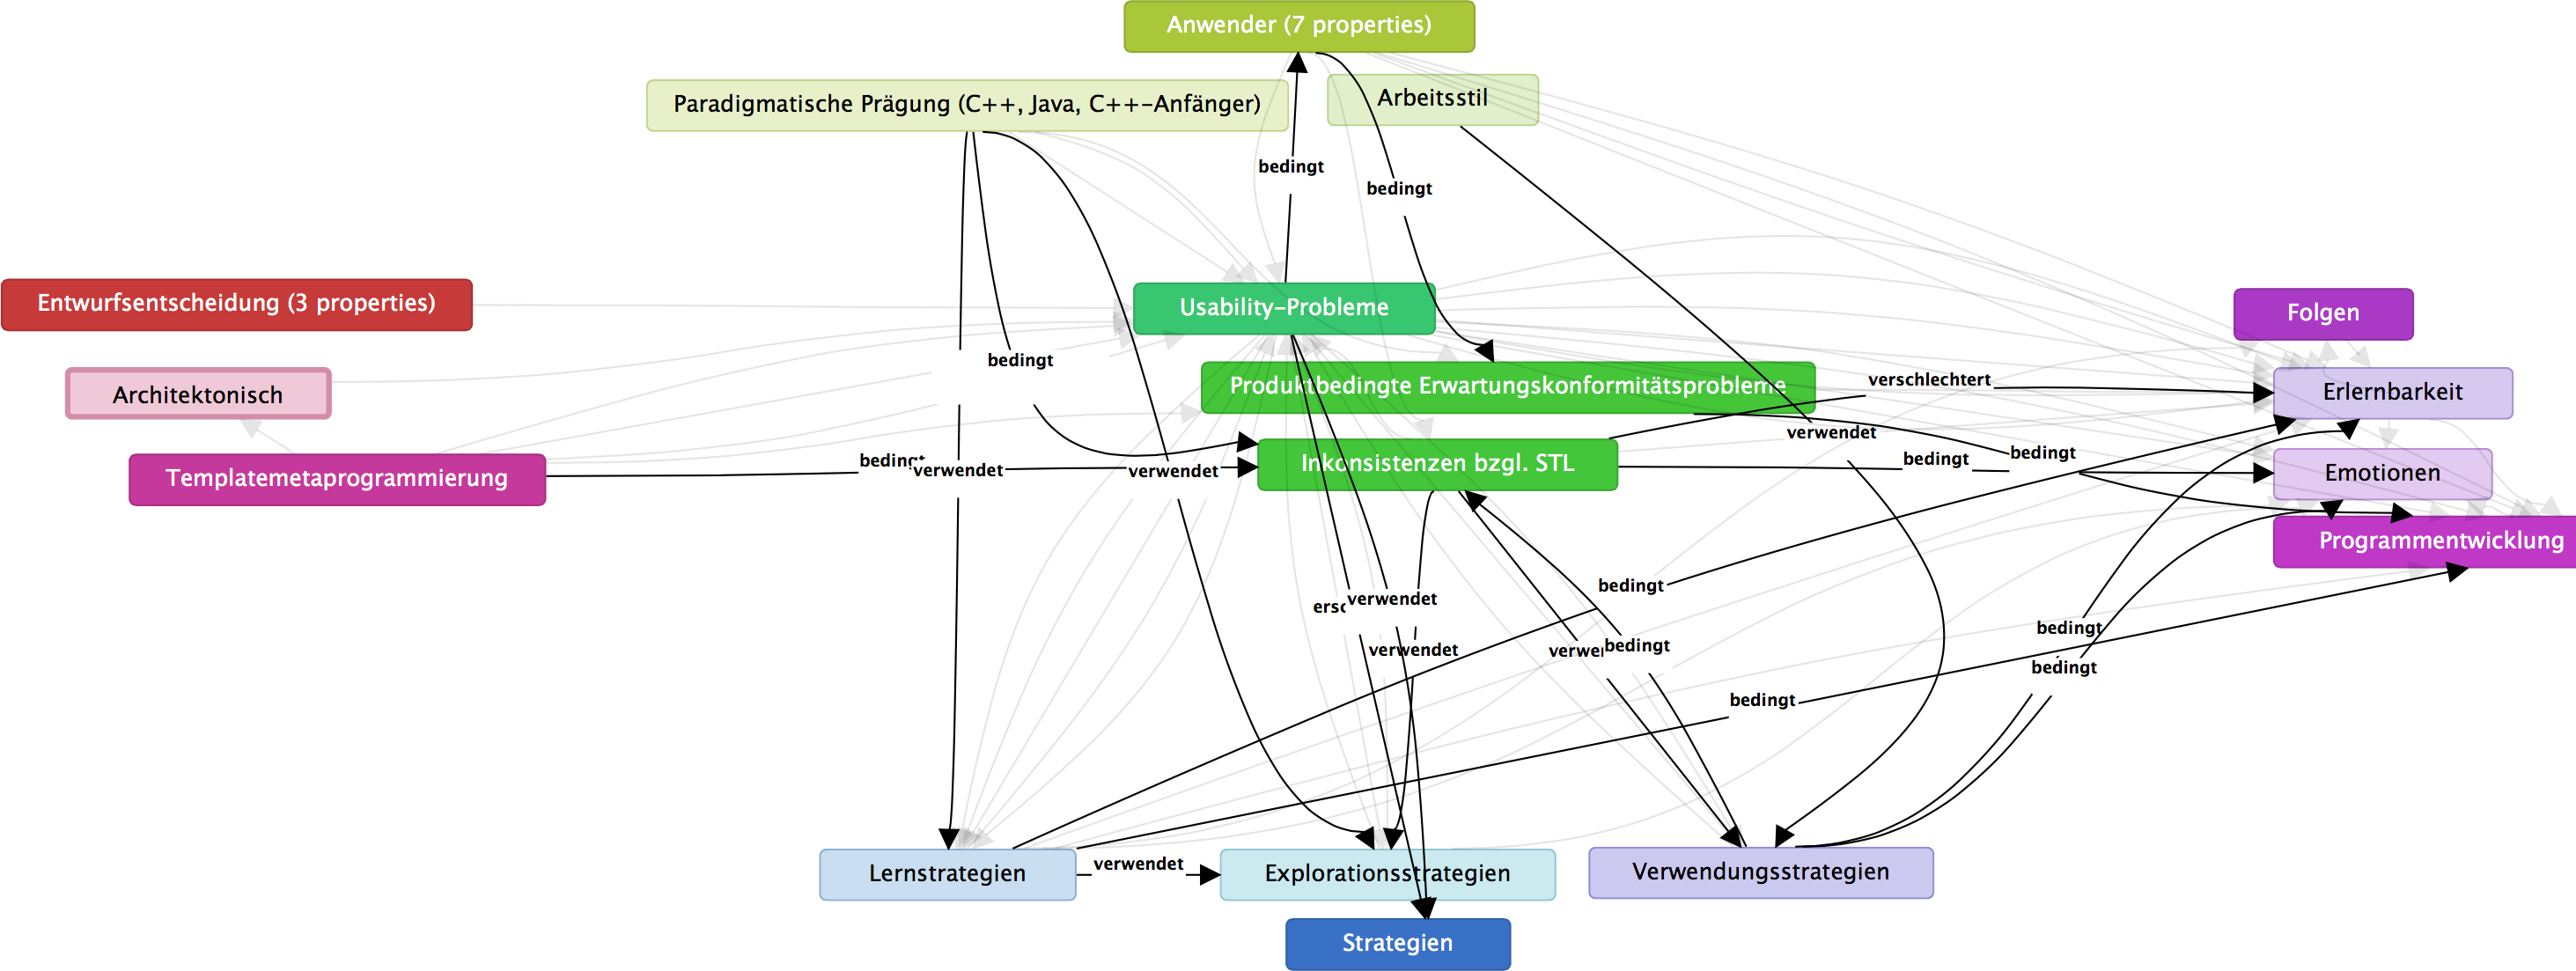
\includegraphics[width=1.0\linewidth]{Figures/research/gt-stl.png}
  \caption{Ursachen und Folgen des Problems \code{apiua://code/-9223372036854775633}}
  \label{fig:research-gt-stl}
\end{minipage}
\end{figure}


\subsubsection{Weiterer Vorschlag: Wrapper-API}
\label{sec:seqan-improve-wrapper-api}

Während ich die Umsetzung des CRTP-Vorschlags mit großer Überzeugung vertreten kann, fehlen mir für den folgenden Vorschlag hinreichend empirisch belegte Erkenntnisse --- siehe \code{apiua://code/-9223372036854775080} bzw. \textit{Java-objektorientierte} \code[apiua://code/-9223372036854775494]{paradigmatische Prägung}.

In der API-Usability-Evaluationsstudie von \cite{Stylos:2008cu} haben die Autoren festgestellt, dass ein Teil der Anwender API-Endanwender sind. Da diese Gruppe andere Anforderungen an eine API stellt, haben sich die Autoren dazu entschlossen, die existierende API nicht zu überarbeiten und damit womöglich die API-Usability für die technischen API-Anwender zu verschlechtern. Stattdessen haben sie eine auf der existierenden API aufbauende Wrapper-API geschaffen, die sich dadurch auszeichnet, dass sie API-Endanwender-zentrisch entwickelt wurde. Sie verfügt über ein weitaus höheres Abstraktionsniveau und verringert die Konfrontation mit technischen Belangen wie Thread-Sicherheit. Auf diese Weise verfügt die verbesserte Library nun über zwei aufeinander aufbauende APIs --- eine für API-Anwender und eine für API-Endanwender.

Dasselbe tat der Workshop'14-Teilnehmer John Reid im Zuge einer Arbeit \citep{Reid:R1ZT4-2v}, bei der SeqAn eingesetzt wurde. Auf Grund Reids großer Unzufriedenheit mit SeqAn\citepurl{bibtex://Reid:R1ZT4-2v}, implementierte er einen Python-basierten SeqAn-API-Wrapper mit Hilfe der \textit{Boost.Python}-Library\footnote{\url{http://www.boost.org/libs/python/}}. Dieser aufwändige Schritt unterstreicht zugleich die Fatalität der dazugehörigen Usability-Probleme. Der Wrapper sieht in seiner Anwendung wie folgt aus:
\begin{minted}[linenos=false]{python}
# Create a set of strings
seqs = seqan.StringDNASet(('ACGT', 'AAAA', 'GGGG', 'AC'))

# Create an enhanced suffix array
index = seqan.IndexStringDNASetESA(seqs)

# Traverse the array (DFS)
it = index.topdownhistory()
it.goBegin()
while not it.atEnd:
  print it.numOccurrences, it.representative
  it.goNext()
\end{minted}

Bereits bei dem ersten SeqAn-Workshop im Jahre 2011 äußerten einzelne Workshop-Teilnehmer im Rahmen der Feedback-Runde den Wunsch, SeqAn in ihre Python-Projekte verwenden zu können. Dieser Wunsch wurde jedoch schnell von Teilen der anwesenden SeqAn-Entwickler wegdiskutiert und nicht weiter verfolgt.

Die Arbeit von \cite{Stylos:2008cu} zeigt, dass es durchaus Sinn machen kann, verschiedene APIs für verschiedene Anwendergruppen zu implementieren. \cite{Reid:R1ZT4-2v} zeigte wiederum, dass eine zweite API möglich ist und wie sie objektorientiert aussehen kann, ohne Performanceverluste zu erleiden.

Erst spät wurde mir klar, dass der VIP-Förderantrag selbst eine solche Wrapper-API vorsah --- ohne sie als solches zu benennen. Die Rede ist von der Workflow-Engine KNIME, auf die ich bereits in den Abschnitten \ref{sec:rahmenbedingungen} und \ref{sec:argument-parser} eingegangen bin. KNIME erlaubt es, als visuelle Knoten gekapselte Programme grafisch zu verknüpfen und auf diese Weise Workflows zu erstellen (siehe \fref{fig:knime}). Eines der Ziele des ebenfalls im \sref{sec:rahmenbedingungen} vorgestellten BioStore-Projekts bestand in der Bereitstellung von SeqAn-Anwendungen innerhalb von KNIME. Es handelt sich dabei also um ein vom BioStore-Projekt erklärtes Ziel, das ich nun auf der Grundlage meiner Forschungsergebnisse unterstütze, weil es sich dabei um eine grafische Wrapper-API handelt, die sich besonders gut für API-Endanwender eignet \citep[vgl.][]{Ko:2004fc,Ko:2011el}. 

\begin{figure}
  \centering
    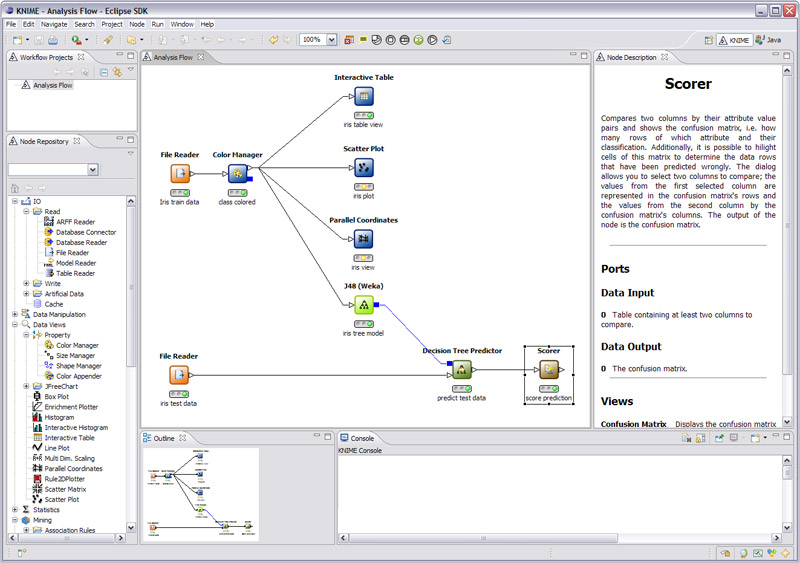
\includegraphics[width=0.8\linewidth]{Figures/knime.jpg}
  \caption{Workflow-Engine KNIME}
  \label{fig:knime}
\end{figure}




\subsection{Maßnahme: Intransparenzbeseitigung}
\textbf{Nutzen:} gering\footnote{Nur ein Anwender schilderte dieses Problem --- allerdings mit Vehemenz. Ich kann daher den genauen Nutzen nicht beurteilen.}; \textbf{Kosten:} mittel

Der Problem der \code[apiua://code/-9223372036854775057]{versteckten Parameterübergabe} muss durch eine explizite Parameterübergabe gelöst werden, was ich an dem folgenden Beispiel verdeutlichen möchte:

\begin{minted}[linenos=false,autogobble=false]{cpp}
typedef Index<DnaString, IndexQGram<UngappedShape<3> > > TIndex;
TIndex index("CATGATTACATA");
hash(indexShape(index), "CAT");
for (unsigned i = 0; i < length(getOccurrences(index, indexShape(index))); ++i)
  std::cout << getOccurrences(index, indexShape(index))[i] << std::endl; 
return 0;
\end{minted}

Dieses Beispiel könnte verbessert lauten:
\begin{minted}[linenos=false,autogobble=false]{cpp}
typedef Index<DnaString, IndexQGram<UngappedShape<3> > > TIndex;
TIndex index("CATGATTACATA");
TShape shape = indexShape(index);
THash shapeHash = hash(shape, "CAT");
for (unsigned i = 0; i < length(getOccurrences(index, shape, shapeHash)); ++i)
  std::cout << getOccurrences(index, indexShape(index))[i] << std::endl; 
return 0;
\end{minted}

In diesem Beispiel habe ich die Rückgaben der Funktionen \texttt{indexShape} und \texttt{hash} expliziert.

Da ich nur durch einen Proband auf dieses Problem aufmerksam wurde, dieses Thema in der API-Usability-Forschung nach meiner Kenntnis unerforscht ist und ich mich mit zeitlichen Problemen konfrontiert sah, habe ich diese Maßnahme nicht weiter verfolgt. Das mit dieser Maßnahme adressierte Problem \code[apiua://code/-9223372036854775057]{versteckte Parameterübergabe} ist jedoch Teil meines Ausblicks.




\subsection{Maßnahme: Inkonsistenzbeseitigung}
\textbf{Nutzen:} hoch; \textbf{Kosten:} hoch

\begin{itemize}
  \item \textit{Indirekte} \code[apiua://code/-9223372036854774918]{Datenstrukturmodifikationen} wie \mintinline{cpp}{fn(x) = 1} und \mintinline{cpp}{fn(fm(x), 1)} müssen durch \textit{direkte-explizite} Datenstrukturmodifikationen wie \mintinline{cpp}{x = 1} oder \mintinline{cpp}{x = fn(y)} ersetzt werden. \textit{Direkte-implizite} Datenstrukturmodifikationen wie \mintinline{cpp}{fn(x, 1)} sind tolerabel, wenn der Funktionsname auf eine Datenstrukturveränderung hinweist (z.B. \mintinline{cpp}{assignValue(x, 1)}).
  
  Auf diese Weise kann das Problem \code{apiua://code/-9223372036854775116} gelöst werden.
  
  \item Zusätzlich müssen Funktionen --- wenn kein dringender Grund dagegen spricht --- Referenzen zurückgeben und der Zuweisungsoperator entsprechend überschrieben werden, um das Problem der \code{apiua://code/-9223372036854774846} zu beheben.
  
%  \item \code{apiua://code/-9223372036854775533}: Wenn schon Shortcuts, dann konsistent (\mintinline{cpp}{String<AminoAcid>} => \mintinline{cpp}{AminoAcidString}) Get/Set nur theoretisch gesehen. Auswirkungen auf Usability-Probleme nicht weiter verfolgt. Daher keine Aussagen.

  \item In SeqAn werden Termini aus verschiedenen Domänen verwendet. Rein fachliche Termini wie \textit{Peptide} dürfen nur dann verwendet werden, wenn tatsächlich eine domänenentsprechende Kapselung mit Mehrwert zur benannten Datenstruktur zu Grunde liegt. Damit wird die Fatalität der Probleme \code{apiua://code/-9223372036854774861} und \code{apiua://code/-9223372036854775623} verringert.
\end{itemize}









\subsection{Maßnahme: Shortcuts}
\textbf{Nutzen:} mittel; \textbf{Kosten:} gering

\code{apiua://code/-9223372036854775611} sind ein Quell der Unmut und haben einen zweifelhaften Nutzen.

\begin{itemize}
  \item Der Name eines Shortcuts sollte sich aus den Bestandteilen ergeben, die es synonymisiert. Damit wird die Wahrscheinlichkeit verringert, dass Shortcuts eine \code[apiua://code/-9223372036854774861]{Abstraktion suggerieren}.
%  \item Der Name eines Shortcuts muss sich auf konsistente Weise ergeben, um einen Aspekt der \code{apiua://code/-9223372036854775533} zu beseitigen.
  \item Offensichtliche Shortcuts sollten entfernt werden oder zumindest nicht in für API-Anwender sichtbaren Code --- insbesondere Code-Beispielen --- verwendet werden. Dadurch kann das Problem \code{apiua://code/-9223372036854774860} gelöst werden.
\end{itemize}









\subsection{Maßnahme: Fail-Fast}
\textbf{Nutzen:} mittel; \textbf{Kosten:} gering

Die \code{apiua://code/-9223372036854775615} hat zwei Ursachen und muss daher auch auf zweierlei Weise gelöst werden:
\begin{enumerate}
  \item Globale (Meta-)Funktionen, die tatsächlich Interface-(Meta-)Funktionen sind, müssen auch als solche implementiert werden. Standardimplementierungen, die auch für ungeeignete Eingaben Werte zurückgeben, müssen beseitigt werden (z.B. \texttt{length}).
  \item Leseoperationen müssen die Möglichkeit zur Verfügung stellen, Lesefehler in Erfahrung zu bringen. Da Performance ein wichtiges Entwurfsziel von SeqAn ist, schlage ich vor, standardmäßig eine Verifikation der eingelesenen Daten vorzunehmen. Anwendern, die nicht bereit sind, diesen Performanceverlust hinzunehmen, muss die Möglichkeit gegeben werden, diese Verifikation zu deaktivieren (z.B. mit Hilfe von \texttt{Tags}).
  
  Ich schlage vor, eine Ausnahme im Falle eines Lesefehlers zu werfen. Der SeqAn-Core-Entwickler Manuel Holtgrewe begrüßte diesen Vorschlag bereits. 
\end{enumerate}


\subsection{Maßnahme: Dokumentation}\label{sec:dox}
\textbf{Nutzen:} hoch; \textbf{Kosten:} hoch

\code{apiua://code/-9223372036854775404} haben neben den \code{apiua://code/-9223372036854775633} die höchste Gesamtfatalität.

Die Dokumentation muss sowohl inhaltlich, als auch technisch überarbeitet werden.

\subsubsection{Inhaltliche Überarbeitung}

\paragraph{Gesamtüberblick}

Die SeqAn-Dokumentation leidet unter ihrem \code[apiua://code/-9223372036854775572]{fehlenden Gesamtüberblick}. Ein solcher muss daher bereitgestellt werden. Er muss folgendes umfassen:
\begin{itemize}
  \item Funktionale Abgrenzung: Was bietet SeqAn an Funktionen an und was nicht?
  \item Entwurf: Wie ``tickt'' SeqAn? Dieser Punkt könnte durch eine Gegenüberstellung eines typischen SeqAn-Programms mit anderen Sprachen erreicht werden. Für die Gegenüberstellung empfehle ich zwei hypothetische, semantisch identische Programme in Java-OOP und ``klassischem'' objektorientierten C\texttt{++}. Beispielsweise könnte die SeqAn-Programmzeile \mintinline{cpp}{resize(score, length(text) - length(pattern) + 1);} in Java \mintinline{java}{score.resize(text.length() - pattern.length() + 1);} lauten. Sobald die Maßnahme \textit{STL-Angleichung} umgesetzt ist, könnte der Vergleich zu C\texttt{++}/STL hinfällig sein.
  \item Entwurfsmotivation: Woher kommen die Unterschiede der Gegenüberstellung? Dieser Abschnitt muss die Motivation des Entwurfs --- beispielsweise durch einen Benchmark --- erläutern, um die Bereitschaft der Anwender zu erhöhen, sich weiterhin mit SeqAn zu befassen und eine höhere Toleranz für SeqAns Entwurf aufzubringen.
\end{itemize}

Eine ausführliche, aber nicht ausschweifende Erläuterung der grundlegenden Entwurfsentscheidungen unterstützt die \code[apiua://code/-9223372036854774821]{Lernstrategie} \code[apiua://code/-9223372036854775163]{konzeptionelles Verstehen}.
    
\paragraph{Beispiele}
\code{apiua://code/-9223372036854775581} behindern eine ganze Reihe von \code[apiua://code/-9223372036854774819]{Explorations-}, \code[apiua://code/-9223372036854774821]{Lern-}, und \code{apiua://code/-9223372036854774820}, was neben meiner Forschung auch die Arbeiten von \cite{Rosson:1996da,Stylos:2006td} für API-Anwender und von \cite{Wiedenbeck:kt,Rosson:2005hw} für API-Endanwender zeigen konnten.

Daher müssen alle nicht-trivialen Dokumentationseinträge über didaktische Code-Beispiele verfügen. Die Code-Beispiele müssen vollständig und voll funktionstüchtig sein, um es Anwendern zu erlauben, die Code-Beispiele ohne Anpassungen ausführen und besser verstehen zu können \citep{Rosson:1996da,Robillard:2010bh}.

\paragraph{Sprachentitätstypen} sind im Kontext von SeqAn ein wichtiges Konzept (siehe \sref{sec:gt-let}, Seite \pageref{sec:gt-let}), da SeqAn wegen seiner \code{apiua://code/-9223372036854775515} eine Fülle neuer \code{apiua://code/-9223372036854775413} einführt, die für SeqAns Anwender auf Grund derer \code[apiua://code/-9223372036854775494]{paradigmatischer Prägungen} unbekannt sind.

Daher schlage ich vor, Sprachentitätstypen explizit in der Dokumentation zu benennen und sämtliche Dokumentationseinträge mit ihrem jeweiligen Sprachentitätstyp zu annotieren. Eine separate Seite soll darüber hinaus alle in SeqAn verwendeten Sprachentitätstypen erläutern.

\paragraph{Punktuelle Verbesserungen}
Zur Lösung des Problems \code{apiua://code/-9223372036854775567} müssen die Unterschiede und Gemeinsamkeiten zwischen ähnlich benannten Typen (z.B. \texttt{String<String>} und \texttt{StringSet}) deutlich erklärt werden.

Eine weiteres Problem ist die \code[apiua://code/-9223372036854775577]{fehlende Dokumentation von Rückgabetypen}. Die Lösung liegt auf der Hand: Jede Erläuterung einer Funktionsrückgabe muss den zurückgegebenen Typ oder die zur Berechnung des Typs notwendige Metafunktion nennen. Damit wird auch gleichzeitig das Problem \code{apiua://code/-9223372036854775513} abgeschwächt.


\subsubsection{Technische Überarbeitung}

\paragraph{Auflistung sämtlicher Funktionen}
Die Dokumentation muss auf Grund der Usability-Probleme \code{apiua://code/-9223372036854775544} und \code{apiua://code/-9223372036854775280} und zur Unterstützung der \code{apiua://code/-9223372036854774819} \code{apiua://code/-9223372036854774900} unter jeder Klasse sämtliche zur Verfügung stehende Member-Funktionen, Interface-Funktionen und Member-Metafunktionen aufführen und klar voneinander unterscheiden. Um den Wartungsaufwand für die Dokumentation zu begrenzen, sollten sich die strukturellen Informationen aus den im Code manifesten Template-Spezialisierungen herleiten.

\paragraph{Suche}
Die \code{apiua://code/-9223372036854775504} innerhalb der Dokumentation muss so angepasst werden, dass sie die Suchergebnisse gewichtet sortiert und auf der Grundlage von Sprachentitätstypen gruppiert.

Das durch das \textit{Vocabulary Problem} bedingte Usability-Problem \code{apiua://code/-9223372036854775623} soll durch die Einführung von Aliassen gelöst werden. So muss beispielsweise der Suchbegriff \texttt{substring} den Dokumentationseintrag \texttt{infix} zu Tage fördern.

Wichtig an dieser Stelle ist die Unterscheidung zwischen den von mir vorgeschlagenen Aliassen und den als problematisch diagnostizierten Shortcuts. Während Shortcuts als eigenständige Entität dokumentiert sind und auch während der Programmierung alternativ genutzt werden können, dienen Aliasse lediglich dazu, unterschiedliche Suchbegriffe für einen bestimmten Dokumentationseintrag zu ermöglichen. Aliasse sind also weder eigenständig dokumentiert, noch können diese in Programmcode verwendet werden. Vielmehr erhöhen sie die Wahrscheinlichkeit eines erfolgreichen Suchtreffers und vermitteln dabei zugleich die in SeqAn verwendete Terminologie.

\paragraph{Fehlerfreiheit}

Die in der Dokumentation und in den \code{apiua://code/-9223372036854775271} verwendeten Code-Beispiele müssen defektfrei sein und kompilieren. Dazu müssen die Beispiele einer Quelle entspringen, die im Sinne der kontinuierlichen Integration (engl. \textit{continuous integration}) getestet wird.



\subsection{Maßnahme: Werkzeugunterstützung}
\textbf{Nutzen:} mittel; \textbf{Kosten:} mittel

Schaut man sich die in \sref{sec:api-tools} vorgestellten API-Werkzeuge an, muss man leider feststellen, dass keines der Arbeiten den Prototypen-Status je verlassen hat oder zumindest nicht als schlüsselfertiges Produkt vorliegt.

Eine Klasse von Werkzeugen unterstützt API-(End-)Anwender bei der Suche von Beispielen. Leider sind alle mir bekannten Lösungen, mit einer Emacs-Ausnahme, als Eclipse-Plugins implementiert. Des Weiteren haben sich die meisten Werkzeuge auf die Programmiersprache Java konzentriert.

Fasst man die Unreife der Werkzeuge, deren IDE- und Sprachabhängigkeit zusammen, muss man leider zu dem Schluss kommen, dass die Kosten für deren Anpassung, ihren Nutzen vermutlich übersteigen.

Die einzige Ausnahme bildet ein Algorithmus von \cite{Buse:2012vv}, der das Problem \code{apiua://code/-9223372036854775581} stark abmildern könnte. Dieser Algorithmus generiert automatisch Code-Beispiele für APIs, die auf typisierten Programmiersprachen basieren. Die Qualität der generierten Code-Beispiele wurde empirisch validiert. Ich halte es für sinnvoll, sich mit diesem Algorithmus näher zu beschäftigen und zu prüfen, mit welchen Kosten eine Anpassung an die Templatemetaprogrammierung-basierte generische Programmierung in C\texttt{++} möglich ist.



\subsection{Maßnahme: Kollaborationsplattform}
\textbf{Nutzen:} mittel; \textbf{Kosten:} mittel

Kollaborationsplattformen wie Webforen haben sich als nützliche Möglichkeit herausgestellt, eine andauernde Kommunikation zwischen API-Entwicklern und -Anwendern zu ermöglichen. Sie stellen eine exzellente Ressource für die Themen Debugging, Bugs und Entwurfsfragen dar. \citep{DaqingHou:2005ba}

Darüber hinaus bergen Webforen das Potential, API-Endanwendern das Wissen und die Hilfe von erfahrenen API-Anwendern zugänglich zu machen. \citep{Ko:2005cl}

Damit handelt es sich um eine relativ global wirkende Maßnahme, die sich dann positiv auf die \code{apiua://code/-9223372036854774824} von SeqAn auswirken sollte, wenn (1) dem Anwender das Problem bekannt ist und (2) der Anwender die Konsultation von Foren nicht scheut. 

Aus diesen Gründen schlage ich die Einrichtung einer Kollaborationsplattform vor.





\subsection{Probleme ohne Lösung}

\code{apiua://code/-9223372036854775100} können nach meiner Kenntnis leider nicht verbessert werden, sondern höchstens durch die Maßnahme \textit{Fail-Fast} verringert werden. Für API-Endanwender käme theoretisch das Debugging-Interface \textit{Whyline} \citep{Ko:2004fc} in Frage. Praktisch scheitert dieser Vorschlag jedoch an der Unreife dieser Lösung und der extrem hohen Kosten für die Anpassung an SeqAn (vgl. \sref{sec:api-tools}). Nur die Aufnahme von \textit{Concepts} in einen der kommenden C\texttt{++}-Sprachstandards könnte nach meiner Einschätzung Abhilfe schaffen.
        
Die \code{apiua://code/-9223372036854775279} besteht darin, dass mindestens zwei Funktionen, die den gleichen Namen tragen, unterschiedliche Dinge tun. Nach \cite{Bloch:2006jk} sollten solche Funktionen unterschiedliche Namen tragen. Dieser Empfehlung stimmen auch SeqAn-Anwender zu. Ungünstigerweise ist die Verwendung generischer --- und damit häufig gleich lautender Namen --- ja gerade das Grundprinzip der \code[apiua://code/-9223372036854775579]{generischen Programmierung}. Würde man die Funktion \texttt{calc} auftrennen in \texttt{calcA} und \texttt{calcB} würde man die \textit{Erweiterbarkeit} einer API massiv beeinträchtigen. Dieses Problem kann also lediglich durch Aufklärung in der Dokumentation teilweise gelöst werden.

Das von mir während meiner Heuristischen Evaluation gefundene Problem der \textit{fehlenden IDE-Integration der Dokumentation} ist der Tatsache geschuldet, dass das aktuelle \textit{DDDoc}-Dokumentationsformat von SeqAn nicht mit dem Dokumentationssystem \textit{Doxygen}\footnote{Es handelt sich dabei um das C\texttt{++}-Pendant zu JavaDoc. Siehe \url{www.doxygen.org}} kompatibel ist. SeqAn hat besondere Anforderungen an das Dokumentationsformat, da es die in SeqAn verwendeten \textit{Concepts} abbilden muss, die noch nicht in den aktuellen C\texttt{++}-Sprachstandard aufgenommen wurden. Jedoch schlage ich unter der Maßnahme Dokumentation eine Änderung des aktuellen Dokumentationsformats vor, die Doxygen ähnelt. Sobald Concepts in den C\texttt{++}-Sprachstandard aufgenommen wurden, sind sehr wahrscheinlich nur noch kleine Anpassungen notwendig, um die Dokumentation in die IDE des Anwenders integrieren zu können.

Die \code[apiua://code/-9223372036854775148]{fehlende Autovervollständigung} ist der \code{apiua://code/-9223372036854775396} von \code[apiua://code/-9223372036854775579]{generischer Programmierung} durch Entwicklungsumgebungen geschuldet. Es ist davon auszugehen, dass die Aufnahme von Concepts in den C\texttt{++}-Sprachstandard zu einer besseren Autovervollständigung führen werden. Diese Entwicklung würde auch den Strategien \code{apiua://code/-9223372036854775145} und \code{apiua://code/-9223372036854774900} entgegen kommen.



\subsection{Weitere Maßnahme: Usability-Priorisierung}
\textbf{Nutzen:} hoch; \textbf{Kosten:} \textit{mittel}

Wie ich bereits im \sref{sec:gt-urursache} angesprochen habe, befindet sich SeqAn gerade dabei, sein Einsatzgebiet auf den kommerziellen Bereich auszuweiten. Diese Entwicklung gibt der zuvor vernachlässigten Usability einen neuen Stellenwert.

SeqAn-Entwickler müssen bei zukünftigen Entwicklungen, wie der Unterstützung von GPUs\footnote{Grafikprozessor ---\textit{Graphics Processing Unit}} und der Parallelisierung von Algorithmen, nun nicht mehr nur Performance und Funktionalität, sondern auch Usability \textit{gleichwertig} miteinander vereinbaren und ihre wissenschaftliche Arbeitsweise ebenfalls auf die Usability übertragen (Stichwort: Usability-Engineering).

Dafür gibt es zwei Gründe:
\begin{enumerate}
  \item Durch die Verwendung eines Consultance-Vermarktungsmodells stehen SeqAn-Entwickler im direkten Kontakt zu ihren Kunden. \textit{Technisches Wegargumentieren} wäre für die Kommunikation mit den Kunden schädlich \citep{Sarodnick:2006vc}.
  \item SeqAn ist zwar eine der schnellsten, aber nicht die einzige Bioinformatik-Softwarebibliothek auf dem Markt. Eine hohe Performance kann eine schlechte Usability nur in Maßen aufwiegen. Tut sie das nicht, wechseln die Kunden zu einem anderen Produkt \citep{sunshine2014searching}. Dies belegen auch meine erhobenen Daten\citepurl{apiua://survey/cd/2013-09-19T11:51:16.616+02:00/provisionality}.  
\end{enumerate}  




\subsection{Zusammenfassung}

In diesem Unterkapitel habe ich Vorschläge zur Verbesserung der API-Usability von SeqAn auf der Grundlage meiner zuvor erhobenen Usability-Probleme und Strategien unterbreitet. Diese Vorschläge sind in Bezug auf die Usability-Probleme weitgehend disjunkt. Die meisten Maßnahmen lassen sich daher hinreichend isoliert bearbeiten.

Die Entwurfsentscheidungen \code{apiua://code/-9223372036854775515} und \code[apiua://code/-9223372036854775579]{generische Programmierung} machen Gebrauch von \textit{Concepts} --- also Interface-ähnlichen Typ-Anforderungsbeschreibungen --- notwendig, von denen SeqAn bereits Gebrauch macht. Allerdings ist in diesem Punkt SeqAn seiner Zeit voraus, denn Concepts sind bis heute nicht in den C\texttt{++}-Sprachstandard aufgenommen worden. Erst C\texttt{++}17 wird voraussichtlich Concepts in die Sprache aufnehmen \citep{Schmidt:2014tf}.

Nach Aufnahme von Concepts in C\texttt{++} ist kurzfristig damit zu rechnen, dass \code{apiua://code/-9223372036854775396} wie die \code[apiua://code/-9223372036854775148]{fehlende Autovervollständigung} und die \code{fehlende IDE-Integration der Dokumentation} entfallen werden. Ich rechne außerdem damit, dass die Lesbarkeit von \code{apiua://code/-9223372036854775100} zunehmen wird, da durch die Unterstützung von Concepts eine Reihe von bisher nur in SeqAn verwendeten \code{apiua://code/-9223372036854775413} auch im Compiler als solche benannt werden.

Mittelfristig rechne ich damit, dass sich die durch Concepts eingeführten neuen \code{apiua://code/-9223372036854775413}, wie \textit{Interface-Funktionen}, innerhalb der C\texttt{++} geprägten Anwenderschaft etablieren werden. Zwar profitieren C\texttt{++} unerfahrene, aber Java-erfahrene Anwender weniger davon, diese werden jedoch bereits durch die Beseitigung der \code{apiua://code/-9223372036854775396} unterstützt.

Die Aufnahme von Concepts in den C\texttt{++}-Sprachstandard bilden also nur einen Baustein bei der Verbesserung der API-Usability von SeqAn.

Die vier wichtigsten Usability-Verbesserungsmaßnahmen sind \begin{itemize}
\itemsep1pt\parskip0pt\parsep0pt
  \item SeqAns Umstellung von einem Framework auf eine Library,
  \item SeqAns Angleichung an die STL,
  \item die Implementierung einer speziell für API-Endanwender entwickelten Wrapper-API und
  \item die Verbesserung der Dokumentation.
\end{itemize}

Ergänzt werden diese Maßnahmen durch punktuellere Maßnahmen wie der Überarbeitung von Shortcuts sowie der Beseitigung von Intransparenzen, Inkonsistenzen und Versagensverschleppungen.

Abschließend habe ich vorgeschlagen, den Dokumentationsaufwand zu begrenzen. Dazu empfiehlt es sich, bereits im Code vorhandene strukturelle Informationen für die Generierung der Dokumentation zu nutzen, das Dokumentationsformat \texttt{DDDoc} syntaktisch zu vereinfachen und den Code-Beispiel-Generationsalgorithmus von \cite{Buse:2012vv} zu evaluieren.

\bigskip

Das nächste Unterkapitel befasst sich mit den bereits erreichten API-Usability-Verbesserungen von SeqAn.